\documentclass[twoside,10pt,twocolumn]{article}
% ------
% Fonts and typesetting settings
\usepackage[sc]{mathpazo}
\usepackage[T1]{fontenc}
\linespread{1.05} % Palatino needs more space between lines

\usepackage{microtype}
% ------
% Page layout
\usepackage[labelfont=bf,labelformat=simple,labelsep=quad]{caption}




\usepackage{graphicx}
\usepackage{amssymb}
\usepackage{epstopdf}
\usepackage{amsfonts}
\usepackage{natbib}
\usepackage{subfigure}
\usepackage{pdfsync}
\usepackage{xspace}
\usepackage{mathrsfs}
\usepackage{fancyhdr}
\usepackage{cuted}
\usepackage{flushend}
\usepackage{url}
%\usepackage{balance}


%% some handy things for making bold math
\def\bm#1{\mathpalette\bmstyle{#1}}
\def\bmstyle#1#2{\mbox{\boldmath$#1#2$}}
\newcommand{\thh}{^\mathrm{th}}


%% Some pretty etc.'s, etc...
\newcommand{\cf}{{\em cf.}\xspace }
\newcommand{\eg}{{\em e.g.},\xspace }
\newcommand{\ie}{{\em i.e.},\xspace }
\newcommand{\etal}{{\em et al.}\ }
\newcommand{\etc}{{\em etc.}\@\xspace}



%% the page dimensions from TeXShop's default---very nice
\textwidth = 6.5 in
\textheight = 9 in
\oddsidemargin = -0.01 in
\evensidemargin = -0.01 in
\topmargin = -0.7 in
\headheight = 0.25 in
\headsep = 0.25 in
\parskip = 0.0in
\parindent = 0.25in

\setlength{\columnsep}{.4in}



%% change section heading styles
\makeatletter
\renewcommand\section{\@startsection {section}{1}{\z@}%
                                   {-3.5ex \@plus -1ex \@minus -.2ex}%
                                   {1.5ex \@plus 0ex}%
                                   {\normalfont\normalsize\bfseries}}
\renewcommand\subsection{\@startsection{subsection}{2}{\z@}%
                                     {-3.25ex\@plus -1ex \@minus -.2ex}%
                                     {1.5ex \@plus .2ex}%
                                     {\normalfont\normalsize\itshape}}
\makeatother


\fancyhead{} % clear all header fields
\chead[]{\vspace*{-.15in}
\includegraphics[width=\textwidth]{images/banner.pdf}}
\cfoot[]{}
\fancyhead[LE]{{\bf \thepage}~~{\sl SUPPORTING INFORMATION FOR:} CIANCIO {\em ET AL.}}
\fancyfoot[RE,LO]{{\footnotesize This supporting information is a US Government work and is in the public domain in the USA.}}
\renewcommand{\headrulewidth}{0pt}


%% Commands for some mathematical notation:
\newcommand{\dates}{\mathscr{D}}
\newcommand{\observ}{\mathscr{O}}
\newcommand{\latent}{\mathscr{L}}
\newcommand{\bz}{\bm{z}}
\newcommand{\btheta}{\bm{\theta}}
\newcommand{\bS}{\bm{S}}



\begin{document}


\pagestyle{fancyplain}



   \begin{strip}
   \mbox{}\\
   \mbox{}\\
        {\LARGE\bf The interoceanic invasion of Chinook salmon in Patagonia, new insights from SNPs\par}
    \mbox{}\\
    \uppercase{Carla Riva-Rossi$^*$, Javier Ciancio$^*$, Eric C. Anderson$^\dagger$, John Carlos Garza$^\dagger$ (I NEED THE FULL AUTHOR
LIST IN THE RIGHT ORDER, STILL)}\\ 
       \mbox{}\\
       
    {\em
    $^*$Centro Nacional Patag�nico--CONICET, Blvd. Brown S/N, (9120) Puerto Madryn, Chubut, Argentina. 
    $^\dagger$Fisheries Ecology Division, 
    Southwest Fisheries Science Center, National Marine Fisheries Service, NOAA, 
    Santa Cruz, CA, USA
    }
    \mbox{}\\
    \mbox{}\\
    Supporting information authored by ERIC C. ANDERSON\\
    Correspondence regarding this supporting information: eric.anderson@noaa.gov\\
    Reproduce these results: \url{https://github.com/eriqande/pata-chinook}
%    \begin{abstract}
%      Boing Boing Boing
%    \end{abstract}
   \end{strip}



\section*{Verifying the utility of {\sc gsi\_sim}}

In the paper, we sought the likely population of origin of fish
in the Caterina River by a variety of means, including by using
a population assignment method implemented in the software {\sc gsi\_sim}
\citep{Andersonetal2008}.  Typically, population assignment is applied in situations
where samples are obtained from mixtures of fish that are all directly and very-recently
descended from a population represented by a sample in the {\em baseline}.  The situation
in the Caterina River is somewhat different because the population in the Caterina river 
may have encountered a relatively large degree of genetic drift from the original progenitor
population and/or the original progenitor population may not be reprented in the baseline.

We conducted simulations to assess the reliability of population assignment in this context.
Specifically, the simulations were designed to verify that:
\begin{enumerate}
\item genetic drift between the time of founding and the time of sampling in the
Caterina was unlikely to lead us to spurious inferences.
\item there are no sources outside of the Lower Columbia and the Willamette reporting 
group areas that would have yielded the results we obtained.
\item even though the exact progenitor population might not be in our baseline, the assignments
back to reporting unit are accurate and can be trusted.
\end{enumerate}

The simulations were conducted as follows: in turn, each of the 68 Chinook populations in the baseline, 
was removed from the baseline, and the allele frequencies in that population were tallied.  Then, six 
new sets of allele frequencies were drawn from the beta distribution to simulate genetic drift at values
of $f = t/(2N_e) \in \{10^{-6}, 0.01, 0.025, 0.05. 0.1, 0.2\}$ where $t$ is number of generations
and $N_e$ is the effective size.
Briefly, if the allele frequency at locus $\ell$ in the removed population was estimated to be $p_\ell$
(we estimated $p_\ell$ in each population as the posterior mean given a uniform prior on 
allele frequency; see for example \citealt{Ran&Mou1997}), then ``drifted`` allele frequencies were simulated by drawing from a beta
distribution with parameters $\alpha$ and $\beta$ defined as 
\begin{eqnarray*}
\alpha &=& p_\ell \frac{1-f}{f} \\
\beta &=&  (1- p_\ell) \frac{1-f}{f}. \\
\end{eqnarray*}
For each of the 6 values of $f$, we simulated 10 new sets of allele frequencies and simulated genotype
data on 76 fish from those new allele frequencies, assuming independence between alleles within and
between loci.  These fish were then assigned to reporting unit using the baseline in which the
focal population had been removed.  We then summarized the output by recording the fraction of fish
simulated from each replicate that were assigned to either the Willamette River, Lower Columbia Spring,
or Lower Columbia Fall reporting units---the three reporting units to which fish in the Caterina
River were assigned.

\chead[]{}
\fancyhead[RO]{{\sl SUPPORTING INFORMATION FOR:} CIANCIO {\em ET AL.}~~{\bf \thepage}}


These simulations effectively allow us to answer the question, ``If the 76 fish sampled in the Caterina 
River were derived from population $X$, but had experienced a degree of genetic drift equal to $f$, then 
what fraction of them would end up being assigned to each of the Willamette River, Lower Columbia 
Spring, or Lower Columbia Fall reporting units?''

The results are summarized in Figure~\ref{fig:main}.  The $y$-axes shows the populations which yielded
at least one simulated fish assigned to either the Willamette River, Lower Columbia 
Spring, or Lower Columbia Fall reporting units, for at least one value of $f$.  The $x$-axes show the 
proportion of fish assigned to each of the three reporting units (color coded as shown in the legend). 
The 6 different facets show results for the 6 different values of~$f$.

The results are very clear.  Only when the fish originated from a Willamette River population, were 
more then 84\% of the fish assigned to the Willamette reporting unit, as in the Caterina River.
Interestingly, as many as 60\% of the fish simulated from the Kalama River with $f= 0.2$ were 
assigned to the Willamette River reporting unit, which may not be surprising given then history
of fish transfers between hatcheries in the region.

In summary, the results {\sc gsi\_sim} obtained in the Caterina River were unlikely to have
occurred without a large fraction of the fish originating from the Willamette River (or possibly
a Lower Columbia stock).  Certainly the results are not consistent with an origin from the Central
Valley of California.



\begin{figure*}
\mbox{} \hspace*{-4.5em}\mbox{}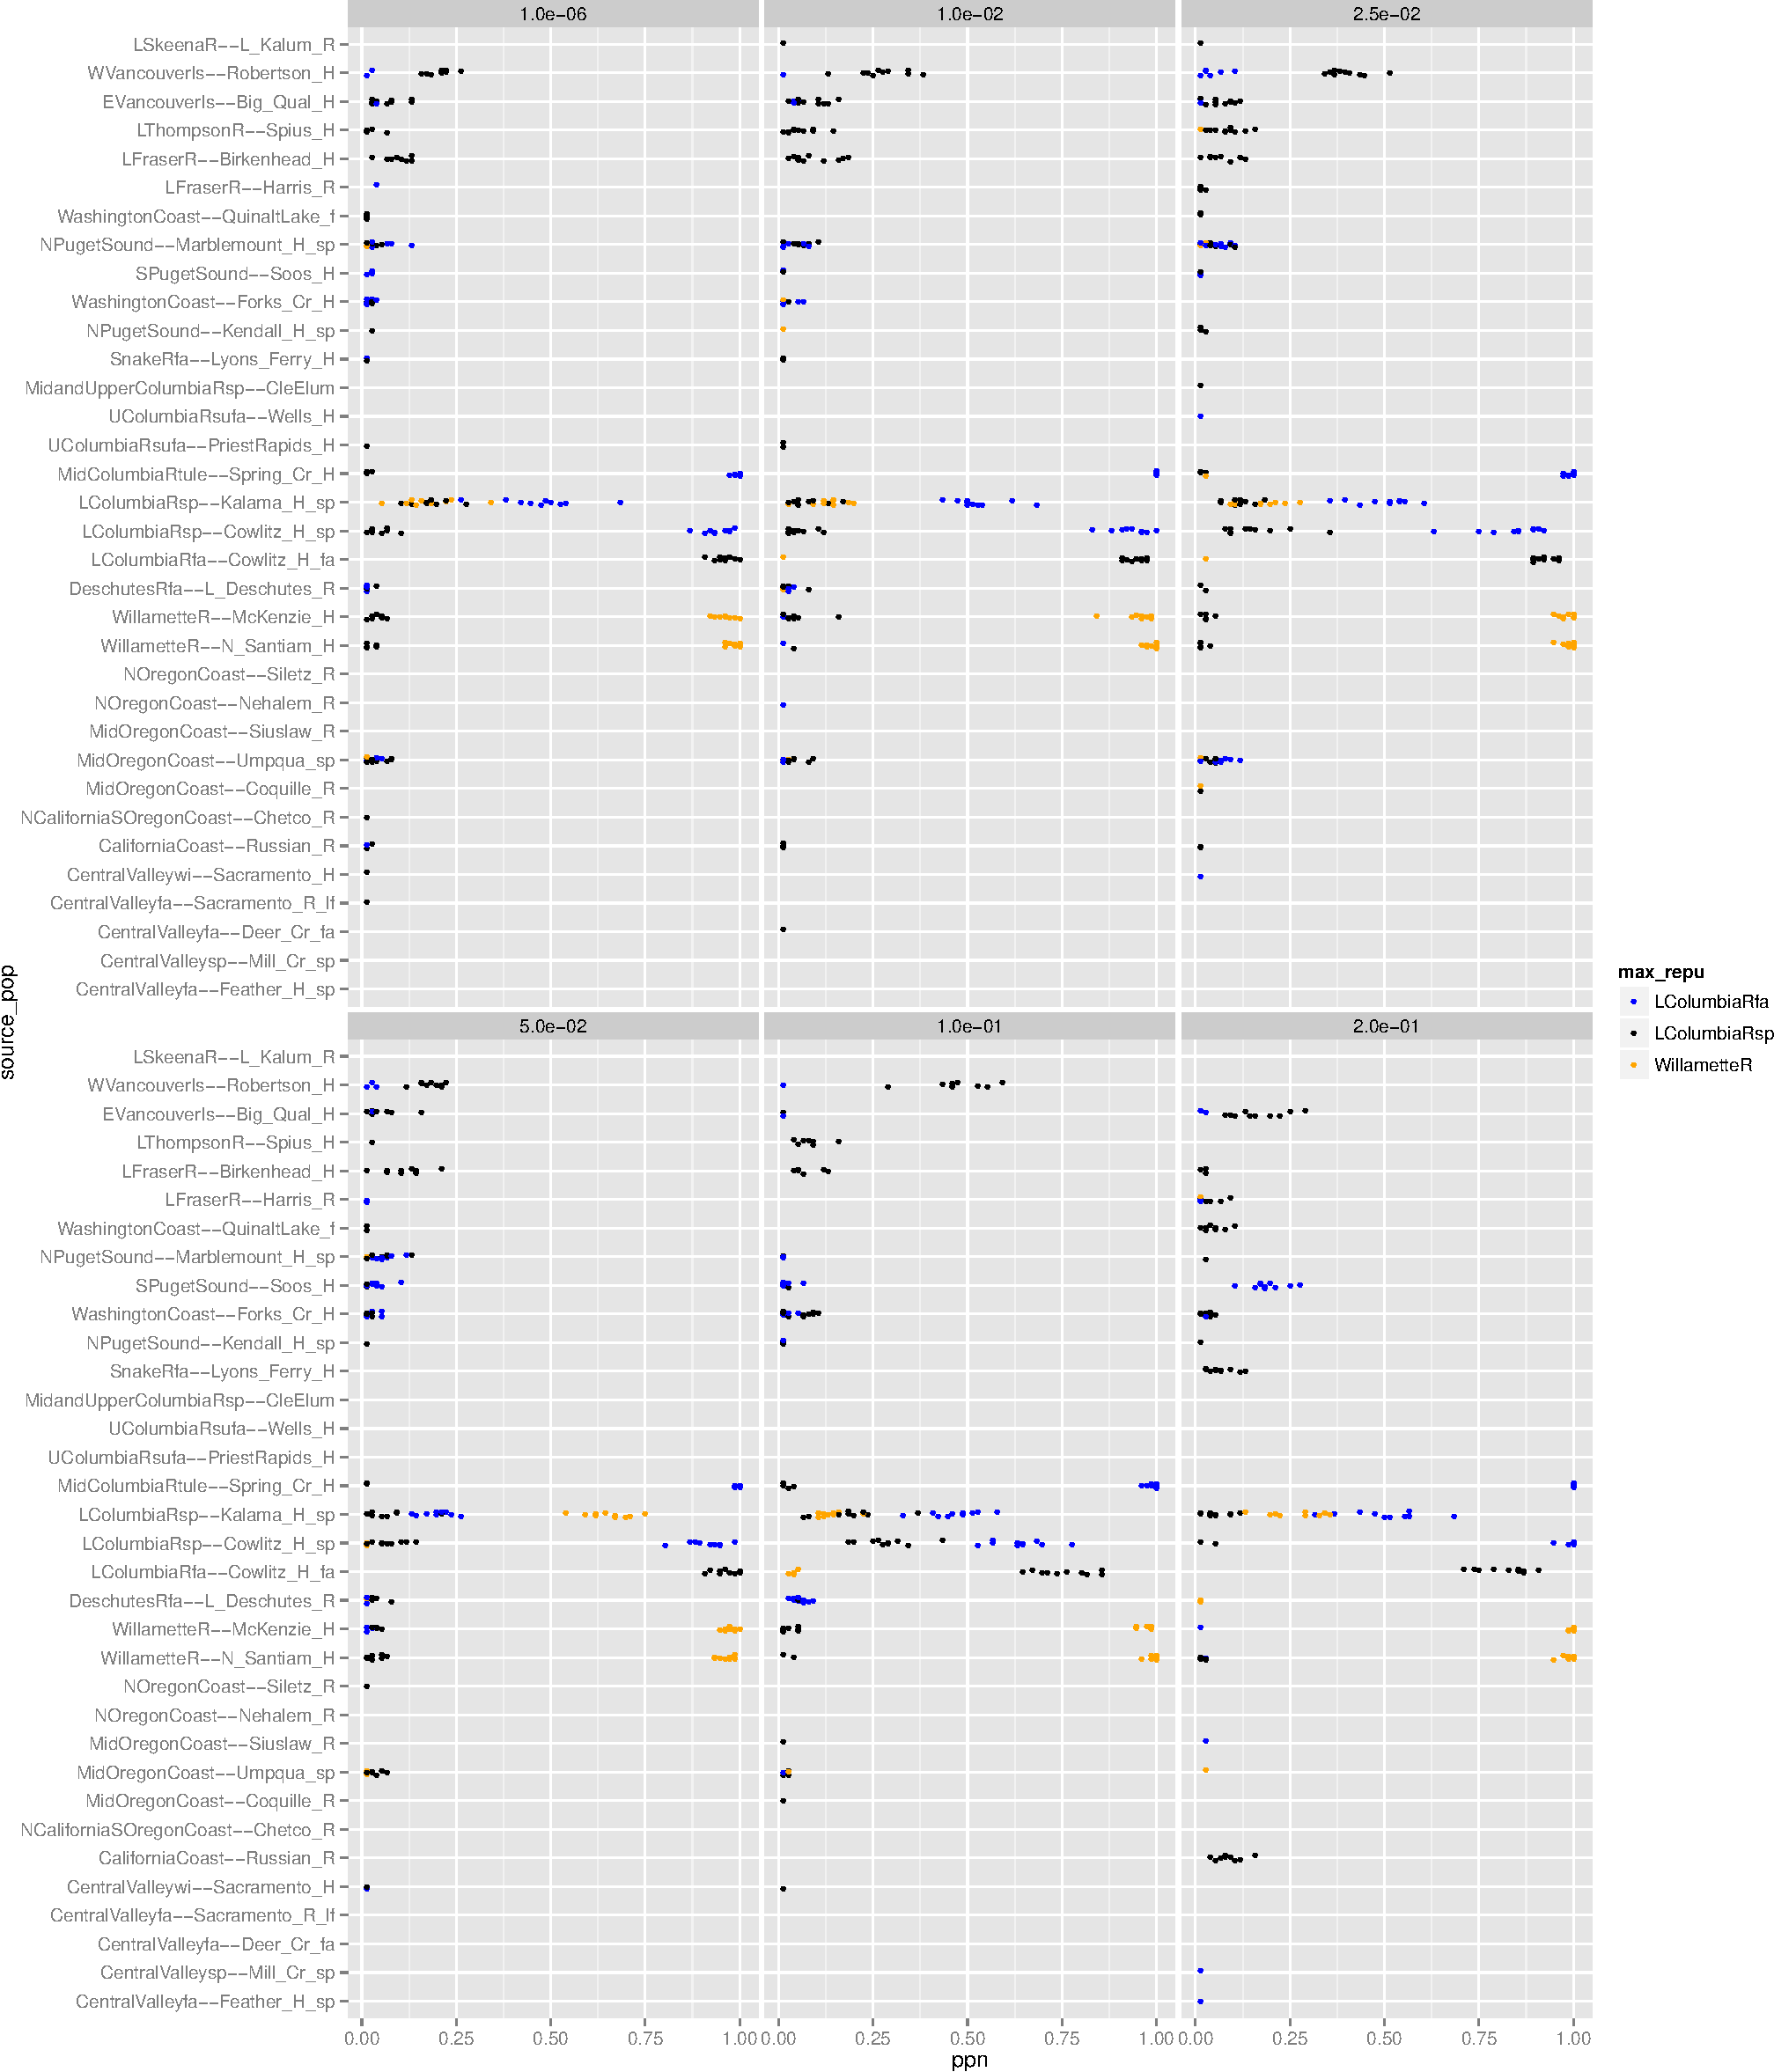
\includegraphics[height = \textheight]{./images/main_fig-crop.pdf}
\caption{See text for explanation}
\label{fig:main}
\end{figure*}

\bibliographystyle{men}
{\footnotesize
\bibliography{pata-chinook}}

 \end{document}
